%!TEX root=../protocol.tex	% Optional

\section{Naměřené hodnoty}
\subsection{Nastavení pulsu}
\begin{figure}[h]
\centering
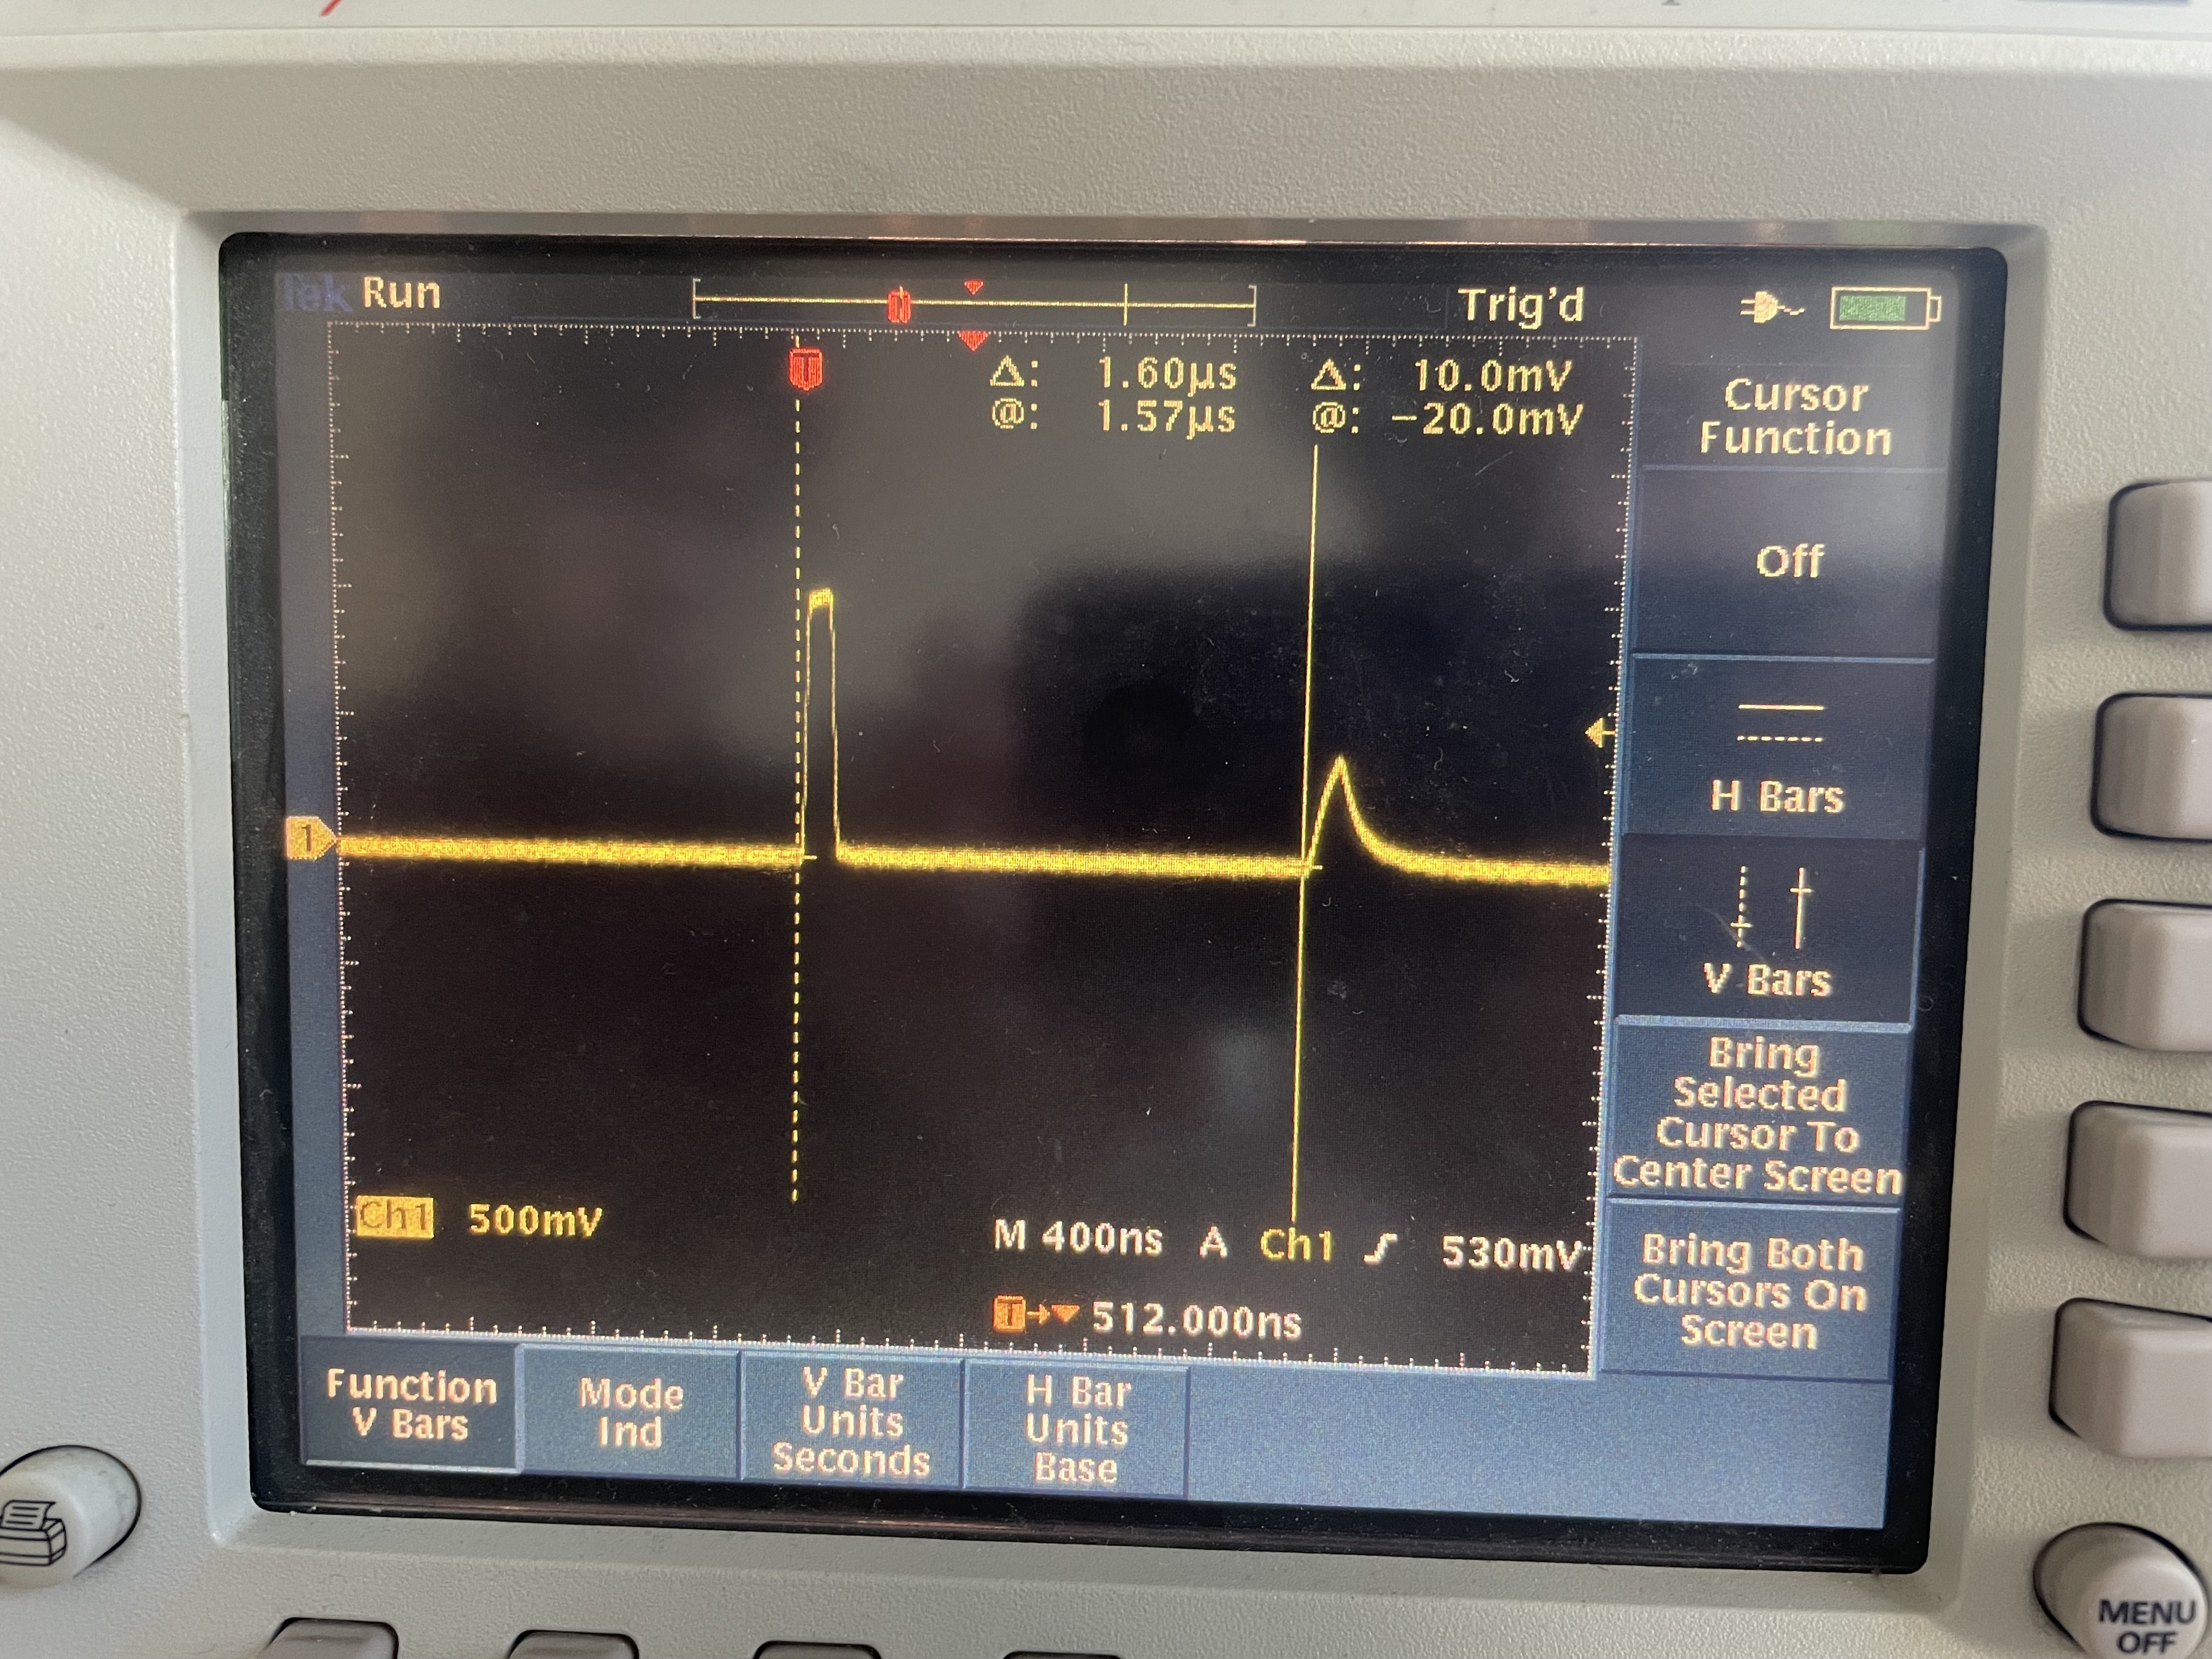
\includegraphics[width=14cm]{images/obr_1.jpg}
\caption{Používaný signál}
\label{fig:5}
\end{figure}

Z toho jsme určili t$=1,6 \cdot 10^{-6}$ s.
\newpage
\subsection{Činitel odrazu na konci vedení}
Nechť činitel odrazu \[\rho_b = \frac{R - Z}{R + Z}\] \\ a mějme $Z=50$ $\Omega$. Pak:

\begin{table}
    \centering
    \caption{Spočítané hodnoty činitele odrazu}
    \begin{tabular}{|c|c|}
       \hline
       R / $\Omega$ & $\rho_b$ / $\Omega$\\
       \hline
       0  & -1\\
       \hline
       25  & -$\frac{1}{3}$\\
       \hline
       50  & 0\\
       \hline
       100  & $\frac{1}{3}$\\
       \hline
       $\infty$ & 1\\
       \hline
    \end{tabular}
    \label{tab:1}
\end{table}
\subsection{Měření délky vedení}
Délka vedení je \[l = 0,65 \cdot c \cdot t \cdot \frac{1}{2}\ \dot{=}\ 0,65 \cdot 3 \cdot 10^{-8} \cdot 1,6 \cdot 10^{-6} \cdot \frac{1}{2}\  \dot{=}\  156\ m.\]
\subsection{Měření impedance vedení}
K odrazu nedochází při odporu $R = 50,3\ \Omega$.
\newpage
\subsection{Data impedančního přizpůsobení}
\begin{figure}[h]
\centering
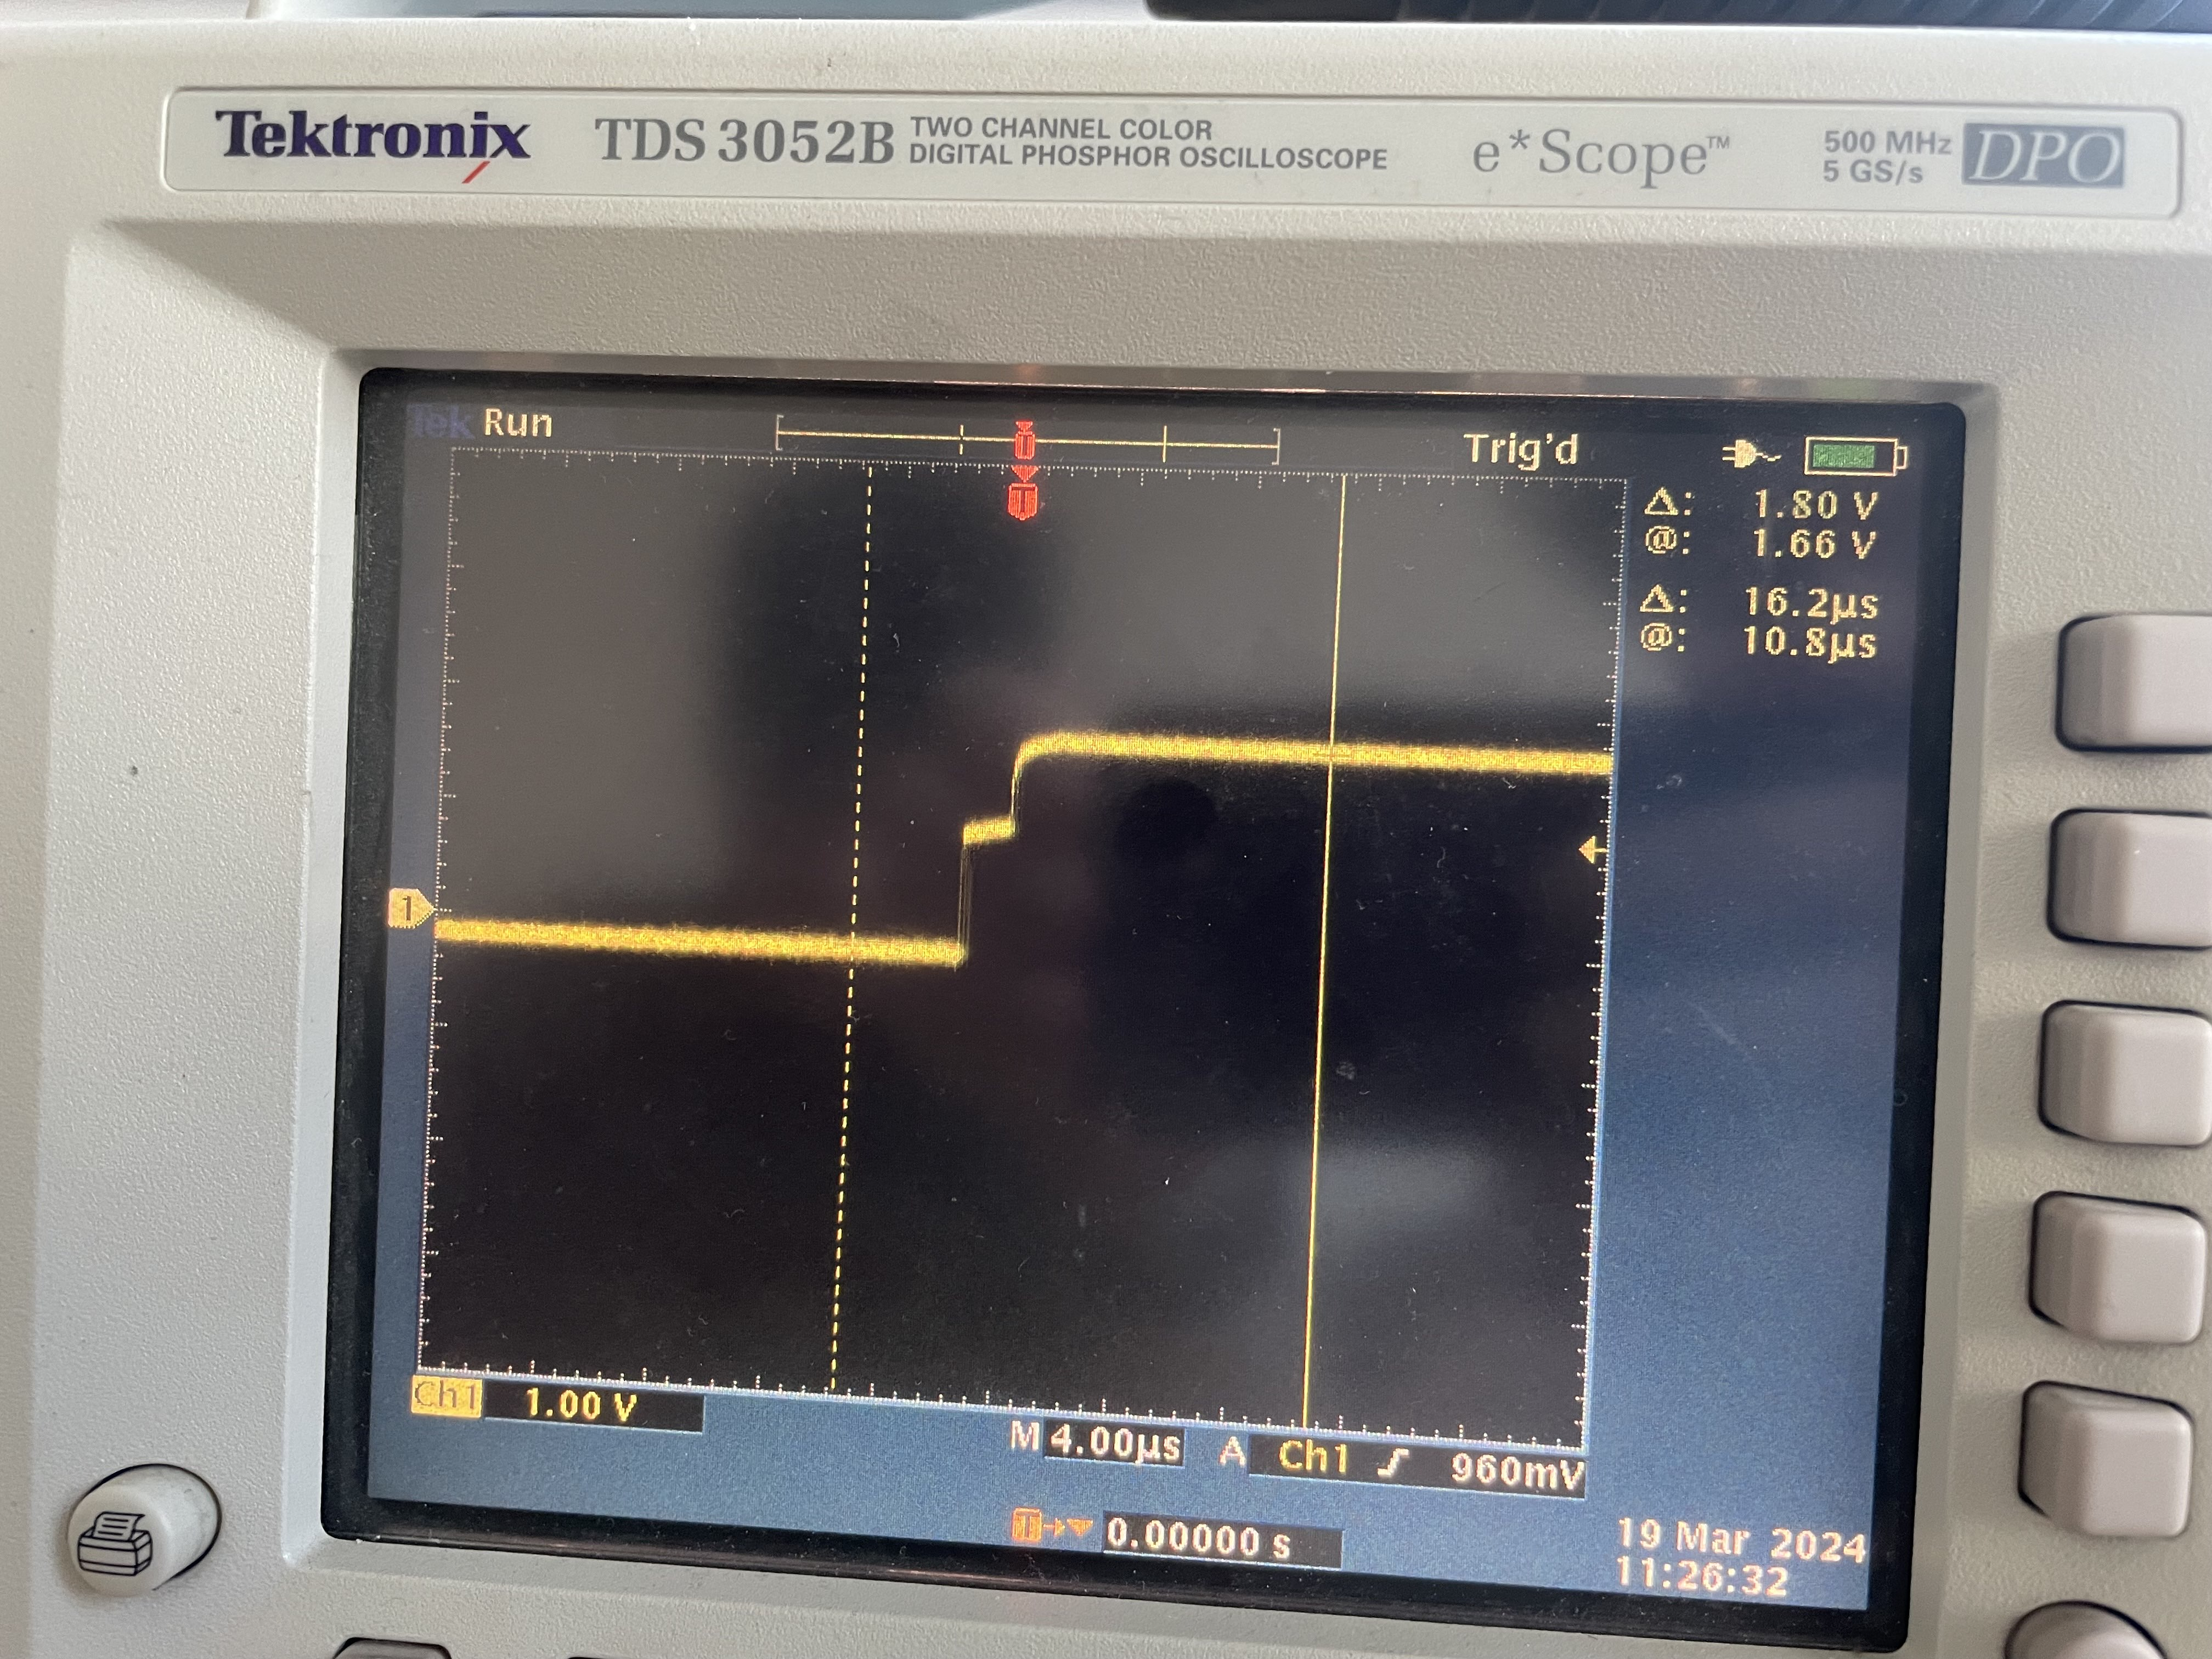
\includegraphics[width=13cm]{images/obr_4.jpg}
\caption{Průběh signálu}
\label{fig:6}
\end{figure}
Signál se nejspíše z části odrazí na začátku vedení, což se zobrazí jako meziskok na osciloskopu.
\section{Zhodnocení}
Během měření jsme si ukázali možnosti využití impedančního přizpůsobení pro detekce různých vad na metalickém vedení. Všechna měření jsme stihli v požadovaném čase i s ohledem na různé pokusy nad rámec zadání.
